\section{Kadek Diva Krishna Murti (1174006)}
\subsection{Pengertian}
\begin{figure}[H]
	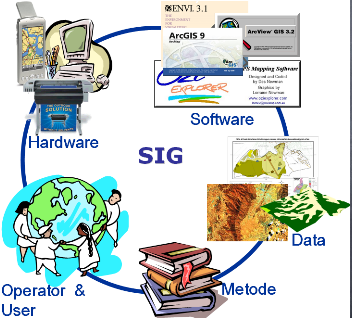
\includegraphics[width=4cm]{figures/1174006/1174006sig1.png}
	\centering
	\caption{Sistem Informasi Geografis.}
\end{figure}
Sistem Informasi Geografis merupakan sebuah runtutan kegiatan yang dilakukan untuk mendapatkan sebuah gambaran mengenai keadaaan ruang muka bumi atau informasi mengenai ruang muka bumi yang dibutuhkan untuk menjawab atau menyelesaikan suatu permasalahan yang ada pada ruang muka bumi yang bersangkutan. Runtutan kegiatan tersebut seperti pengumpulan, penataan, pengolahan, penganalisisan dan penyajian data-data atau fakta-fakta yang terdapat pada ruang muka bumi tertentu. Data atau fakta tersebut disebut sebagai data atau fakta geografis atau data atau fakta spatial. Hasil analisisnya disebut Informasi geografis atau Informasi spatial. Jadi Sistem Informasi Geografis merupakan runtutan kegiatan pengumpulan, penataan, pengolahan dan penganalisisan data atau fakta spatial sehingga diperoleh informasi spasial untuk dapat menjawab atau menyelesaikan suatu permasalahan pada ruang muka bumi tertentu.
\subsection{Sejarah}
\begin{figure}[H]
	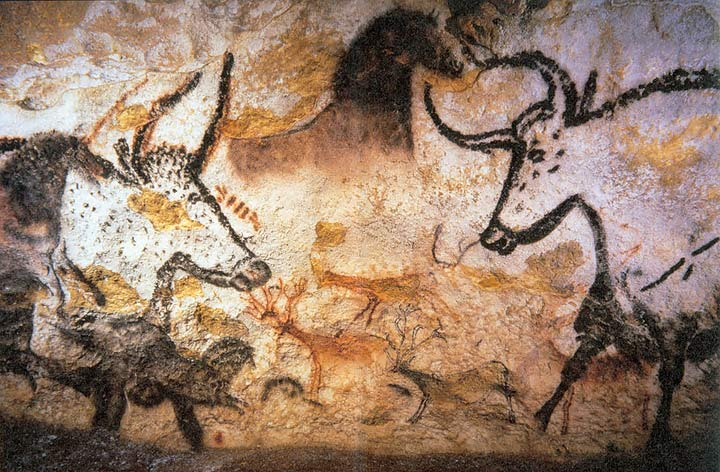
\includegraphics[width=4cm]{figures/1174006/1174006gua1.jpg}
	\centering
	\caption{Gua Lascaux.}
\end{figure}
Pada 35000 tahun yang lalu, di sebuah dinding tepatnya di gua Lascaux, Perancis, para pemburu Cro-Magnon menggambarkan hewan-hewan mangsa mereka. Mereka juga menggambarkan garis-garis yang dipercaya sebagai rute dari migrasi hewan-hewan mangsa mereka tersebut. Catatan awal tersebut sejalan dengan dua elemen struktur pada sistem informasi geografis modern saat ini, arsip grafis yang terhubung ke database atribut. 
Lalu pada tahun 1700-an teknik survei modern untuk pemetaan topografis diterapkan, termasuk versi awal pemetaan tematis, contohnya untuk keilmuan atau data sensus. 
Kemudian pada awal abad ke-20 memperlihatkan pengembangan "litografi foto" dimana peta dipisahkan menjadi beberapa lapisan (layer). Perkembangan perangkat keras komputer yang dipacu oleh penelitian senjata nuklir membawa aplikasi pemetaan menjadi multifungsi pada awal tahun 1960-an. 
Setelah itu, pada tahun 1967 menjadi awal pengembangan sistem informasi geografis yang bisa diterapkan di Ottawa, Ontario oleh Departemen Energi, Pertambangan dan Sumber Daya. Sistem ini dikembangkan oleh Roger Tomlinson, yang kemudian disebut CGIS (Canadian GIS - SIG Kanada) yang digunakan untuk menyimpan, menganalisis dan mengolah data-data yang sebelumnya telah dikumpulkan untuk kepentingan Inventarisasi Tanah di Kanada (CLI - Canadian land Inventory) - dimana ini merupakan sebuah inisiatif untuk mengetahui kemampuan dari suatu lahan yang ada di wilayah pedesaan Kanada dengan cara memetakaan berbagai informasi mengenai tanah, pertanian, pariwisata, alam bebas, unggas dan penggunaan tanah pada skala 1:250000. Faktor pemeringkatan klasifikasi juga diterapkan untuk keperluan analisis.
\begin{figure}[H]
	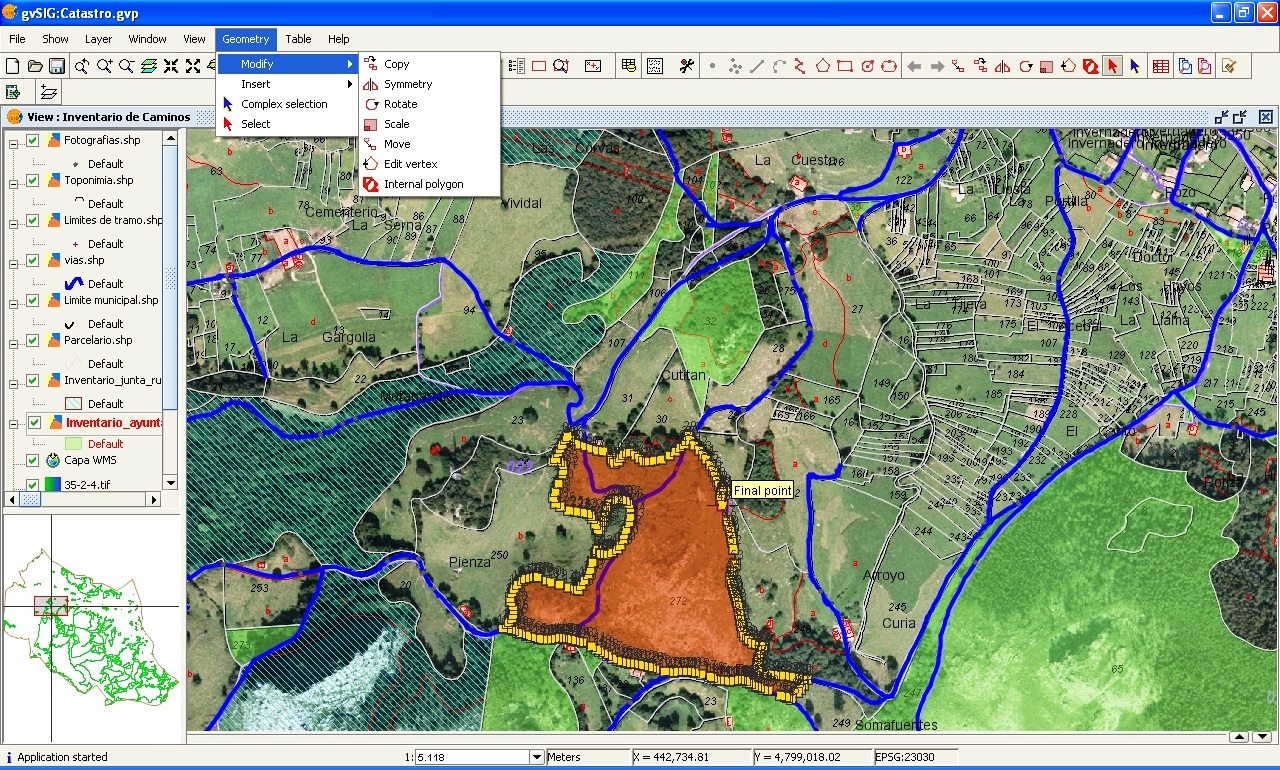
\includegraphics[width=4cm]{figures/1174006/1174006sigapp1.jpg}
	\centering
	\caption{Aplikasi SIG.}
\end{figure}
\subsection{Koordinat}
Koordinat digunakan untuk menunjukkan suatu titik di bumi berdasarkan garis lintang dan garis bujur. Koordinat dibagi menjadi dua bagian irisan yaitu irisan melintang yang disebut dengan garis lintang mulai dari khatulistiwa, membesar ke arah kutub(utara mupun selatan) sedangkanyang lain membujur mulai dari garis Greenwhich membesar ke arah barat dan timur. Satuan skala pada koordinat dibagi menjadi derajat lintang 0\textdegree sampai 90\textdegree dan bujur 0\textdegree sampai 180\textdegree.
Informasi sebuah lokasi didasarkan pada sistem koordinat, yang mencakup datum dan proyeksi peta. Datum adalah kumpulan parameter dan titik kontrol yanghubungan geometriknya diketahui, baik melalui pengukuranatau penghitungan. Sedangkan sistem proyeksi peta adalah sistem yang dirancang untuk merepresentasikan permukaan dari suatu bidang lengkung atau spheroid (misalnya bumi) pada suatu bidang datar. Proses representasi ini menyebabkan distorsi yang perlu diperhitungkan untuk memperoleh ketelitian beberapa macam properti, seperti jarak, sudut, atau luasan.
\begin{figure}[H]
	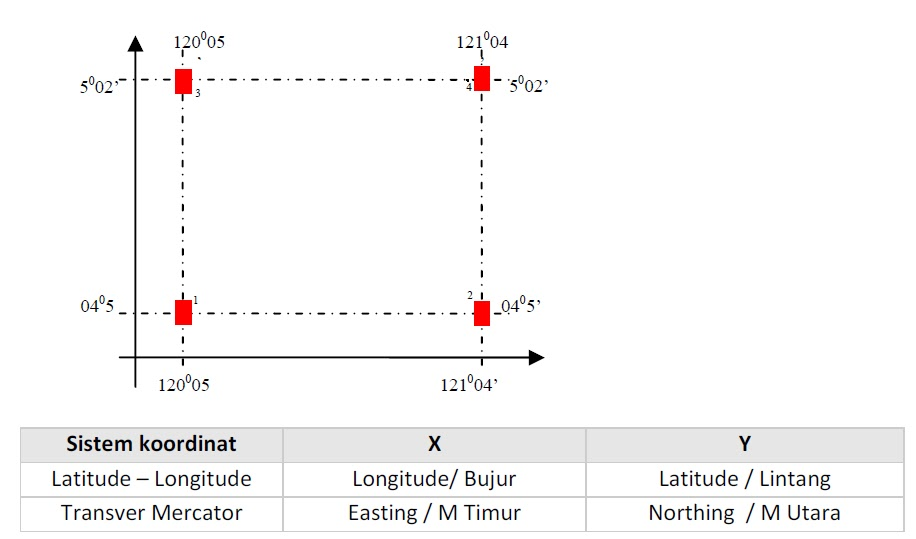
\includegraphics[width=4cm]{figures/1174006/1174006koordinat1.jpg}
	\centering
	\caption{Sistem Koordinat.}
\end{figure}
\subsection{Data Geospasial}
\subsubsection{Data Vektor}
Data vektor adalah data yang direkam dalam bentuk koordinat titik yang menampilkan, menempatkan, dan menyimpan data spasial dengan menggunakan titik, garis atau area (polygon).
\begin{figure}[H]
	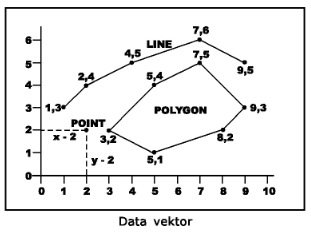
\includegraphics[width=4cm]{figures/1174006/1174006vektor1.png}
	\centering
	\caption{Data Vektor.}
\end{figure}
Ada tipe-tipe data vector yang bisa digunakan untuk menampilkan informasi pada peta. 
\begin{enumerate}
	\item Titik bisa digunakan sebagai lokasi sebuah kota atau posisi tower radio. 
	\item Garis bisa digunakan untuk menunjukkan route suatu perjalanan atau menggambarkan boundary.
	\item Poligon bisa digunakan untuk menggambarkan sebuah danau atau sebuah Negara pada peta dunia.
\end{enumerate}

\subsubsection{Data Raster}
Data raster adalah data yang disimpan dalam bentuk grid atau petak sehingga terbentuk suatu ruang yang teratur dalam bentuk pixel. 
Foto digital seperti areal fotografi atau satelit merupakan bagian dari data raster pada peta.
\begin{figure}[H]
	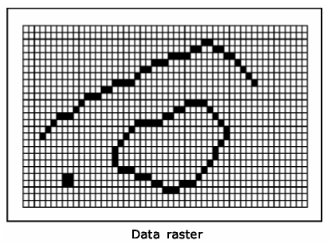
\includegraphics[width=4cm]{figures/1174006/1174006raster1.png}
	\centering
	\caption{Data Raster.}
\end{figure}
Data raster dihasilkan dari sistem penginderaan jauh dan sangat baik untuk merepresentasikan batas-batas yang berubah secara gradual seperti jenis tanah, kelembaban tanah, suhu, dan lain-lain.
Obyek geografis pada data rastel direpresentasikan sebagai struktur sel grid yang disebut sebagai pixel.
Resolusi tergantung pada ukuran pixelnya, semakin kecil ukuran permukaan bumi yang direpresentasikan oleh sel, semakin tinggi resolusinya. Dengan kata lain, resolusi pixel menggambarkan ukuran sebenarnya dipermukaan bumi yang diwakili oleh setiap pixel pada citra.

\subsubsection{Perbedaan Data Vektor dan Data Rastel}
Data vektor relatif lebih ekonomis dalam hal ukuran file dan presisi dalam lokasi. Tetapi sangat sulit untuk digunakan dalam komputasi matematik. Sebaliknya data raster biasanya membutuhkan ruang penyimpanan file yang lebih besar dan presisi lokasinya lebih rendah tetapi lebih mudah digunakan secara matematis.

\subsection{Link}
\href{https://youtu.be/2BjDss7m9SQ}{https://youtu.be/2BjDss7m9SQ}

\subsection{Plagiarism}
\begin{figure}[H]
	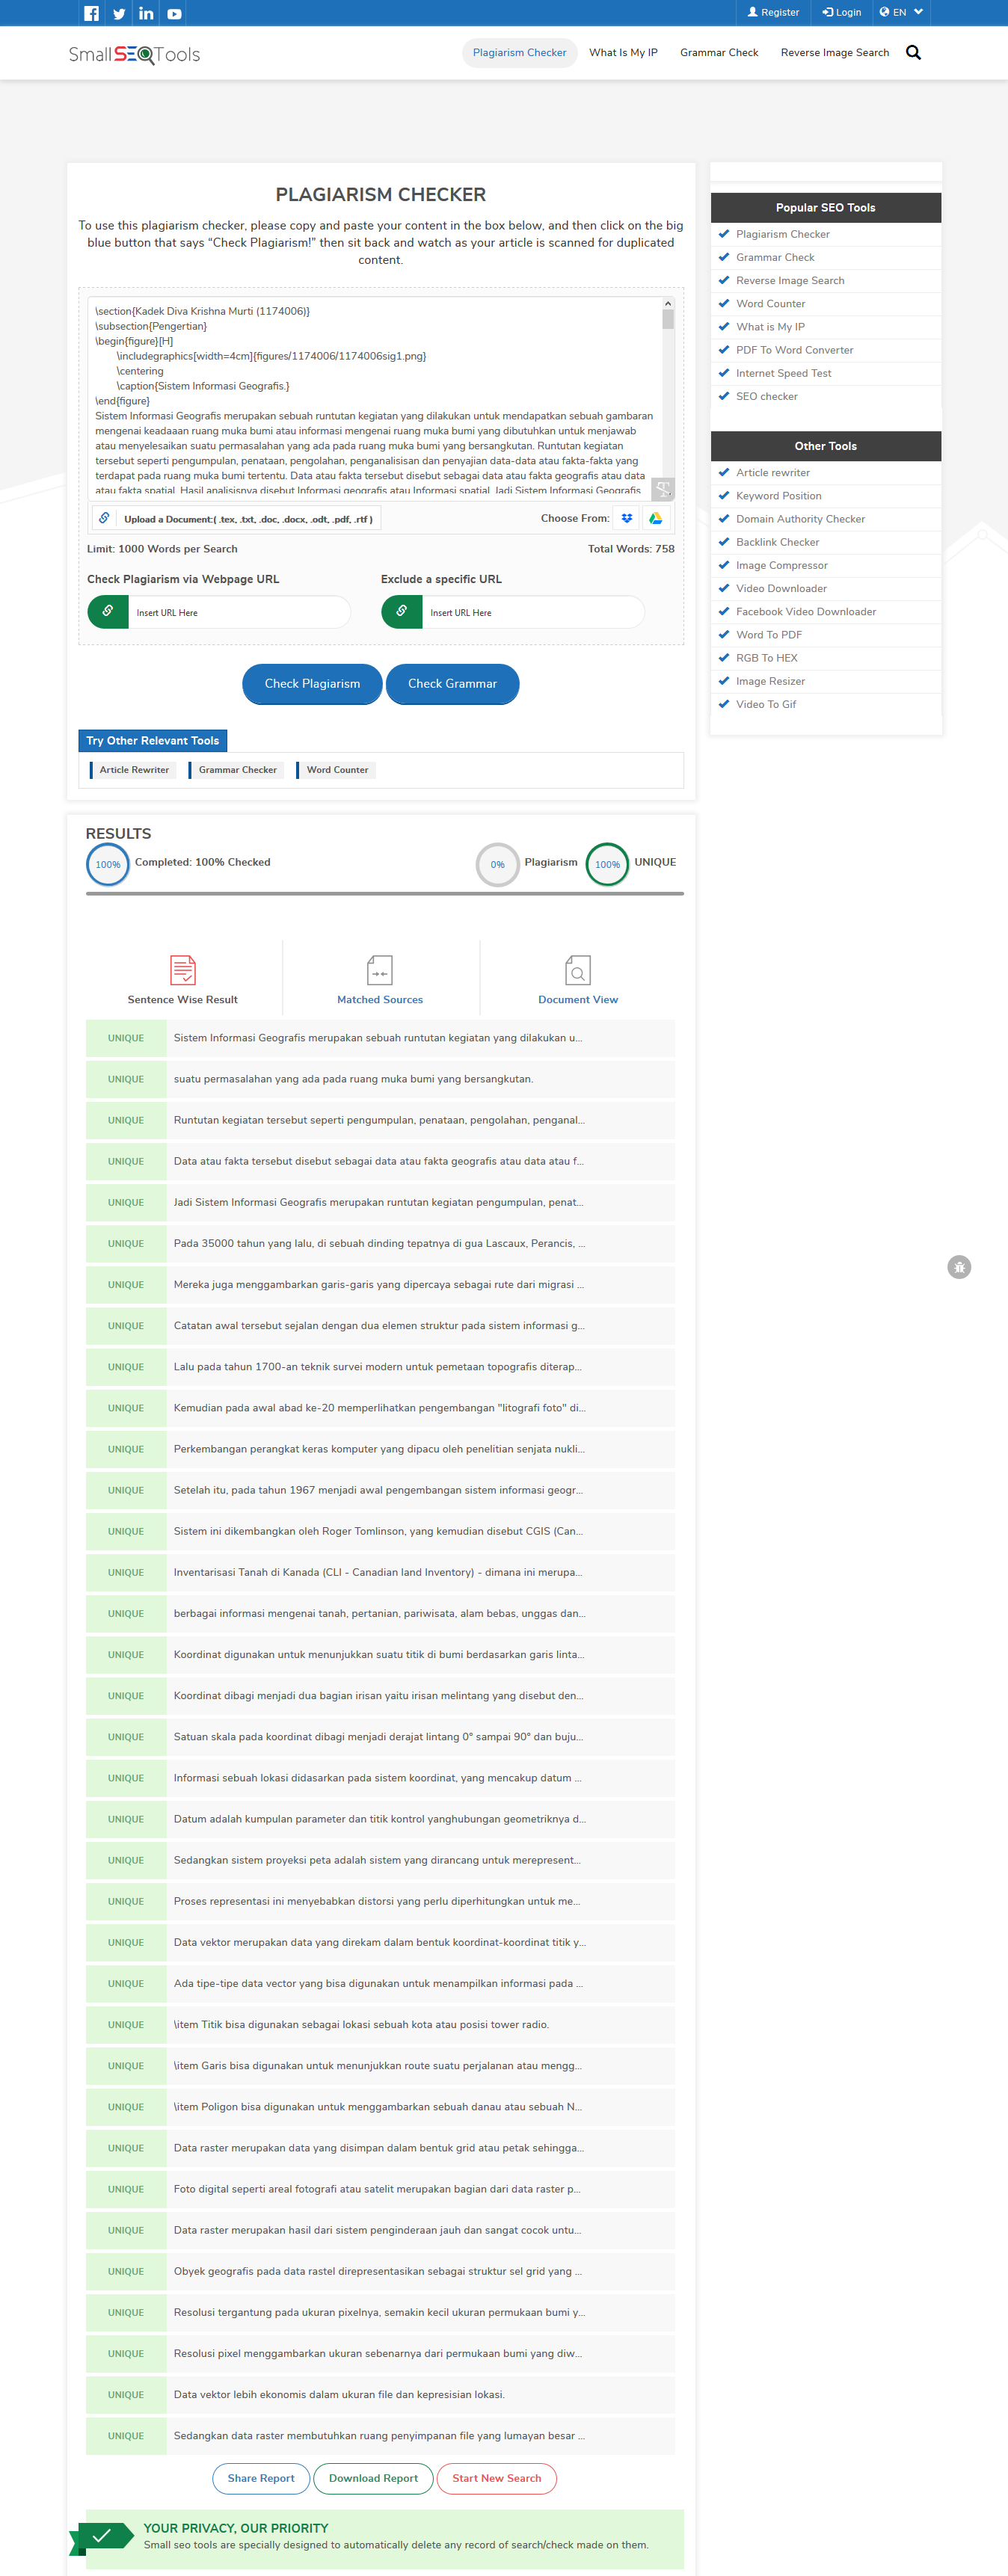
\includegraphics[width=4cm]{figures/1174006/1174006plagiarism1.png}
	\centering
	\caption{Plagiarism 1174006.}
\end{figure}
